\begin{frame}{Frequent Sequential Patterns}{Looking for meaningful frequent patterns in exams sequences}

    \centering\textit{Which exams are "skipped" the most by the students?} \vspace{0,3cm}

\begin{block}{Mining process}
		\begin{itemize}
			\item<1-> \alert{GSP algorithm} --- Apriori-based algorithm to extract frequent sequential patterns from the \emph{students} data;
			\item<2-> \alert{Unusual pattern mining} --- filtering of the GSP output, with the goal of discarding uninteresting (regular) exams patterns;
			\item<3-> \alert{Out-of-place exams mining} --- extraction of the exams that are passed \emph{after} a later exam.
		\end{itemize}
	\end{block}

\end{frame}

\begin{frame}{Associative Rules Analysis}{Looking for implications among the dataset's attributes}

	\vspace{0.3cm}
	Exam names coding and \emph{right order} \tiny{--- it follows the degree course's schedule.}

    \vspace{0.3cm}
    \begin{centering}
        \hspace*{3.0cm}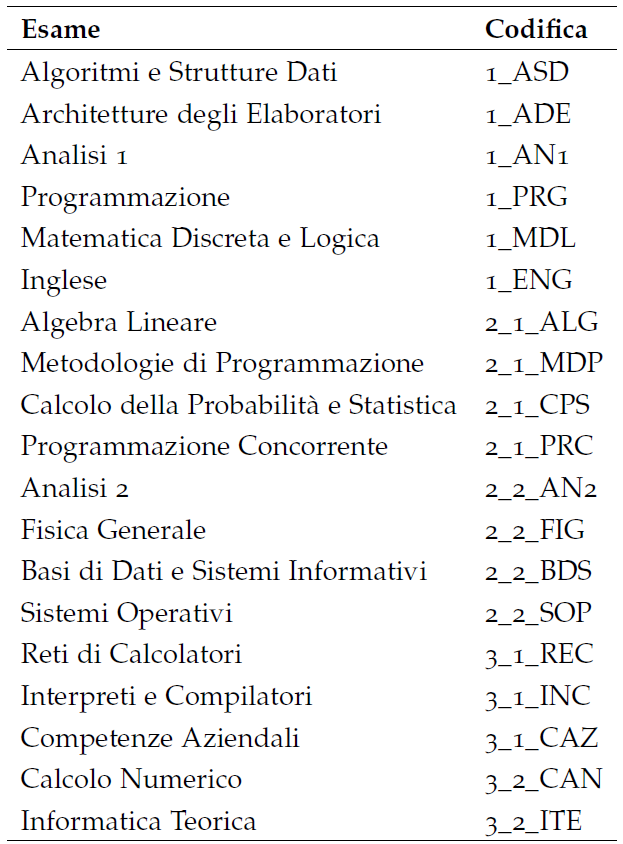
\includegraphics[scale=0.20]{seq1.png}
    \end{centering}

\end{frame}

\begin{frame}{Associative Rules Analysis}{Looking for implications among the dataset's attributes}

    \alert{Example} of a frequent, unusual pattern: \\

	\vspace{0.3cm}
	\begin{centering}
		\texttt{3\_2\_CN, 3\_2\_ITE, 2\_2\_FIG}\\
	\end{centering}
	\vspace{0.3cm}

	... which stands for:

	\vspace{0.3cm}
	\begin{centering}
	\texttt{Calcolo Numerico, Informatica Teorica, Fisica Generale}\\
	\end{centering}
	\vspace{0.6cm}

	\texttt{Fisica Generale} is \alert{out of place}, for it is a $2^{nd}$ year exam done after some $3^r{d}$ year exams.\\

\end{frame}

\begin{frame}{Associative Rules Analysis}{Looking for implications among the dataset's attributes}

   Counting how many times an exams is out of place and making proportions with all out-of-place exams, we get...\\ \vspace{0.5cm}

    \centering\texttt{1\_MDL: 22.16, 1\_ADE: 1.55, 2\_2\_SOP: 0.44, 2\_2\_FIG: 42.72, 2\_1\_MDP: 13.69, 2\_1\_CPS: 1.66, 2\_1\_PRC: 16.39, 2\_1\_ALG: 1.39}

\end{frame}

\begin{frame}{Associative Rules Analysis}{Looking for implications among the dataset's attributes}

	...and displaying that results in a pie diagram:

    \vspace{0.3cm}
    \begin{centering}
        \hspace*{1.0cm}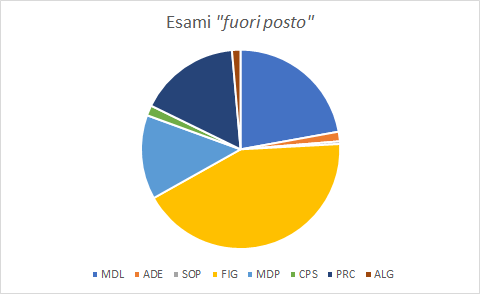
\includegraphics[scale=0.50]{../seq/out_of_place.png}
    \end{centering}

\end{frame}